\documentclass{article}
\usepackage{graphicx}
\begin{document}
	\section*{Lsg Vorschlag Ü09RUT Maximilian Maag}
	\subsection*{Aufgabe 9.1}
	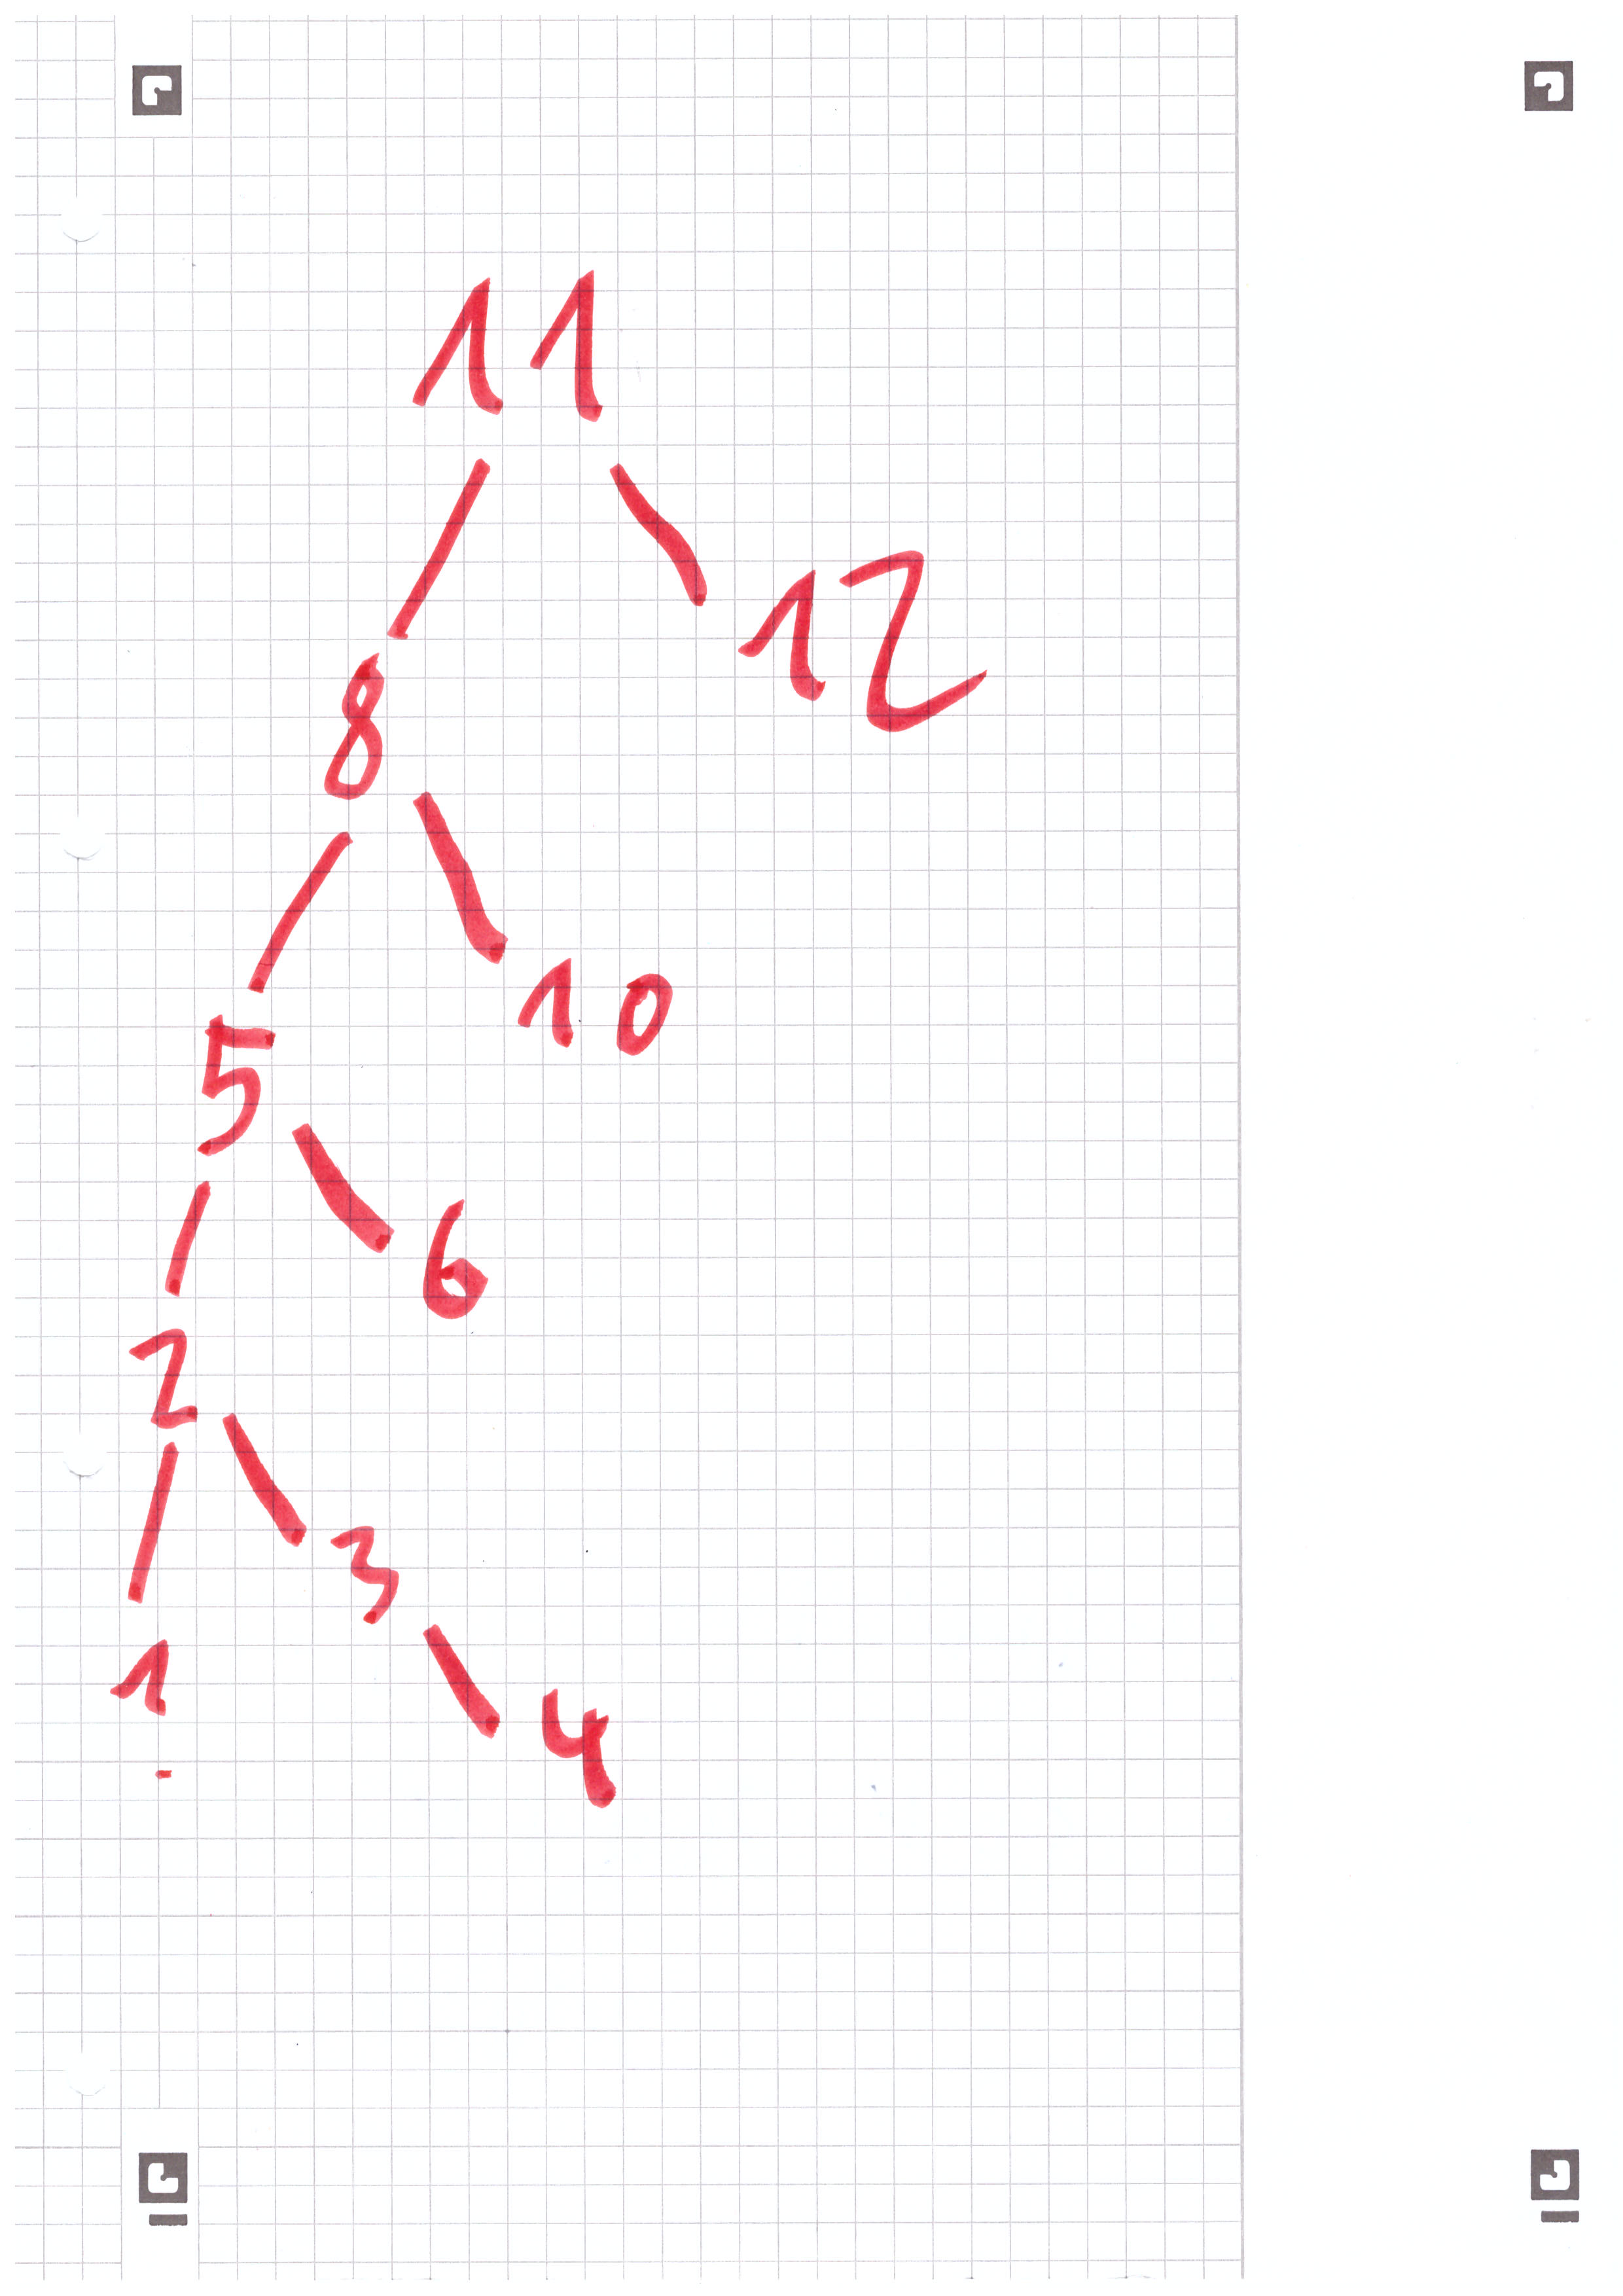
\includegraphics[width=\linewidth]{090101} \\
	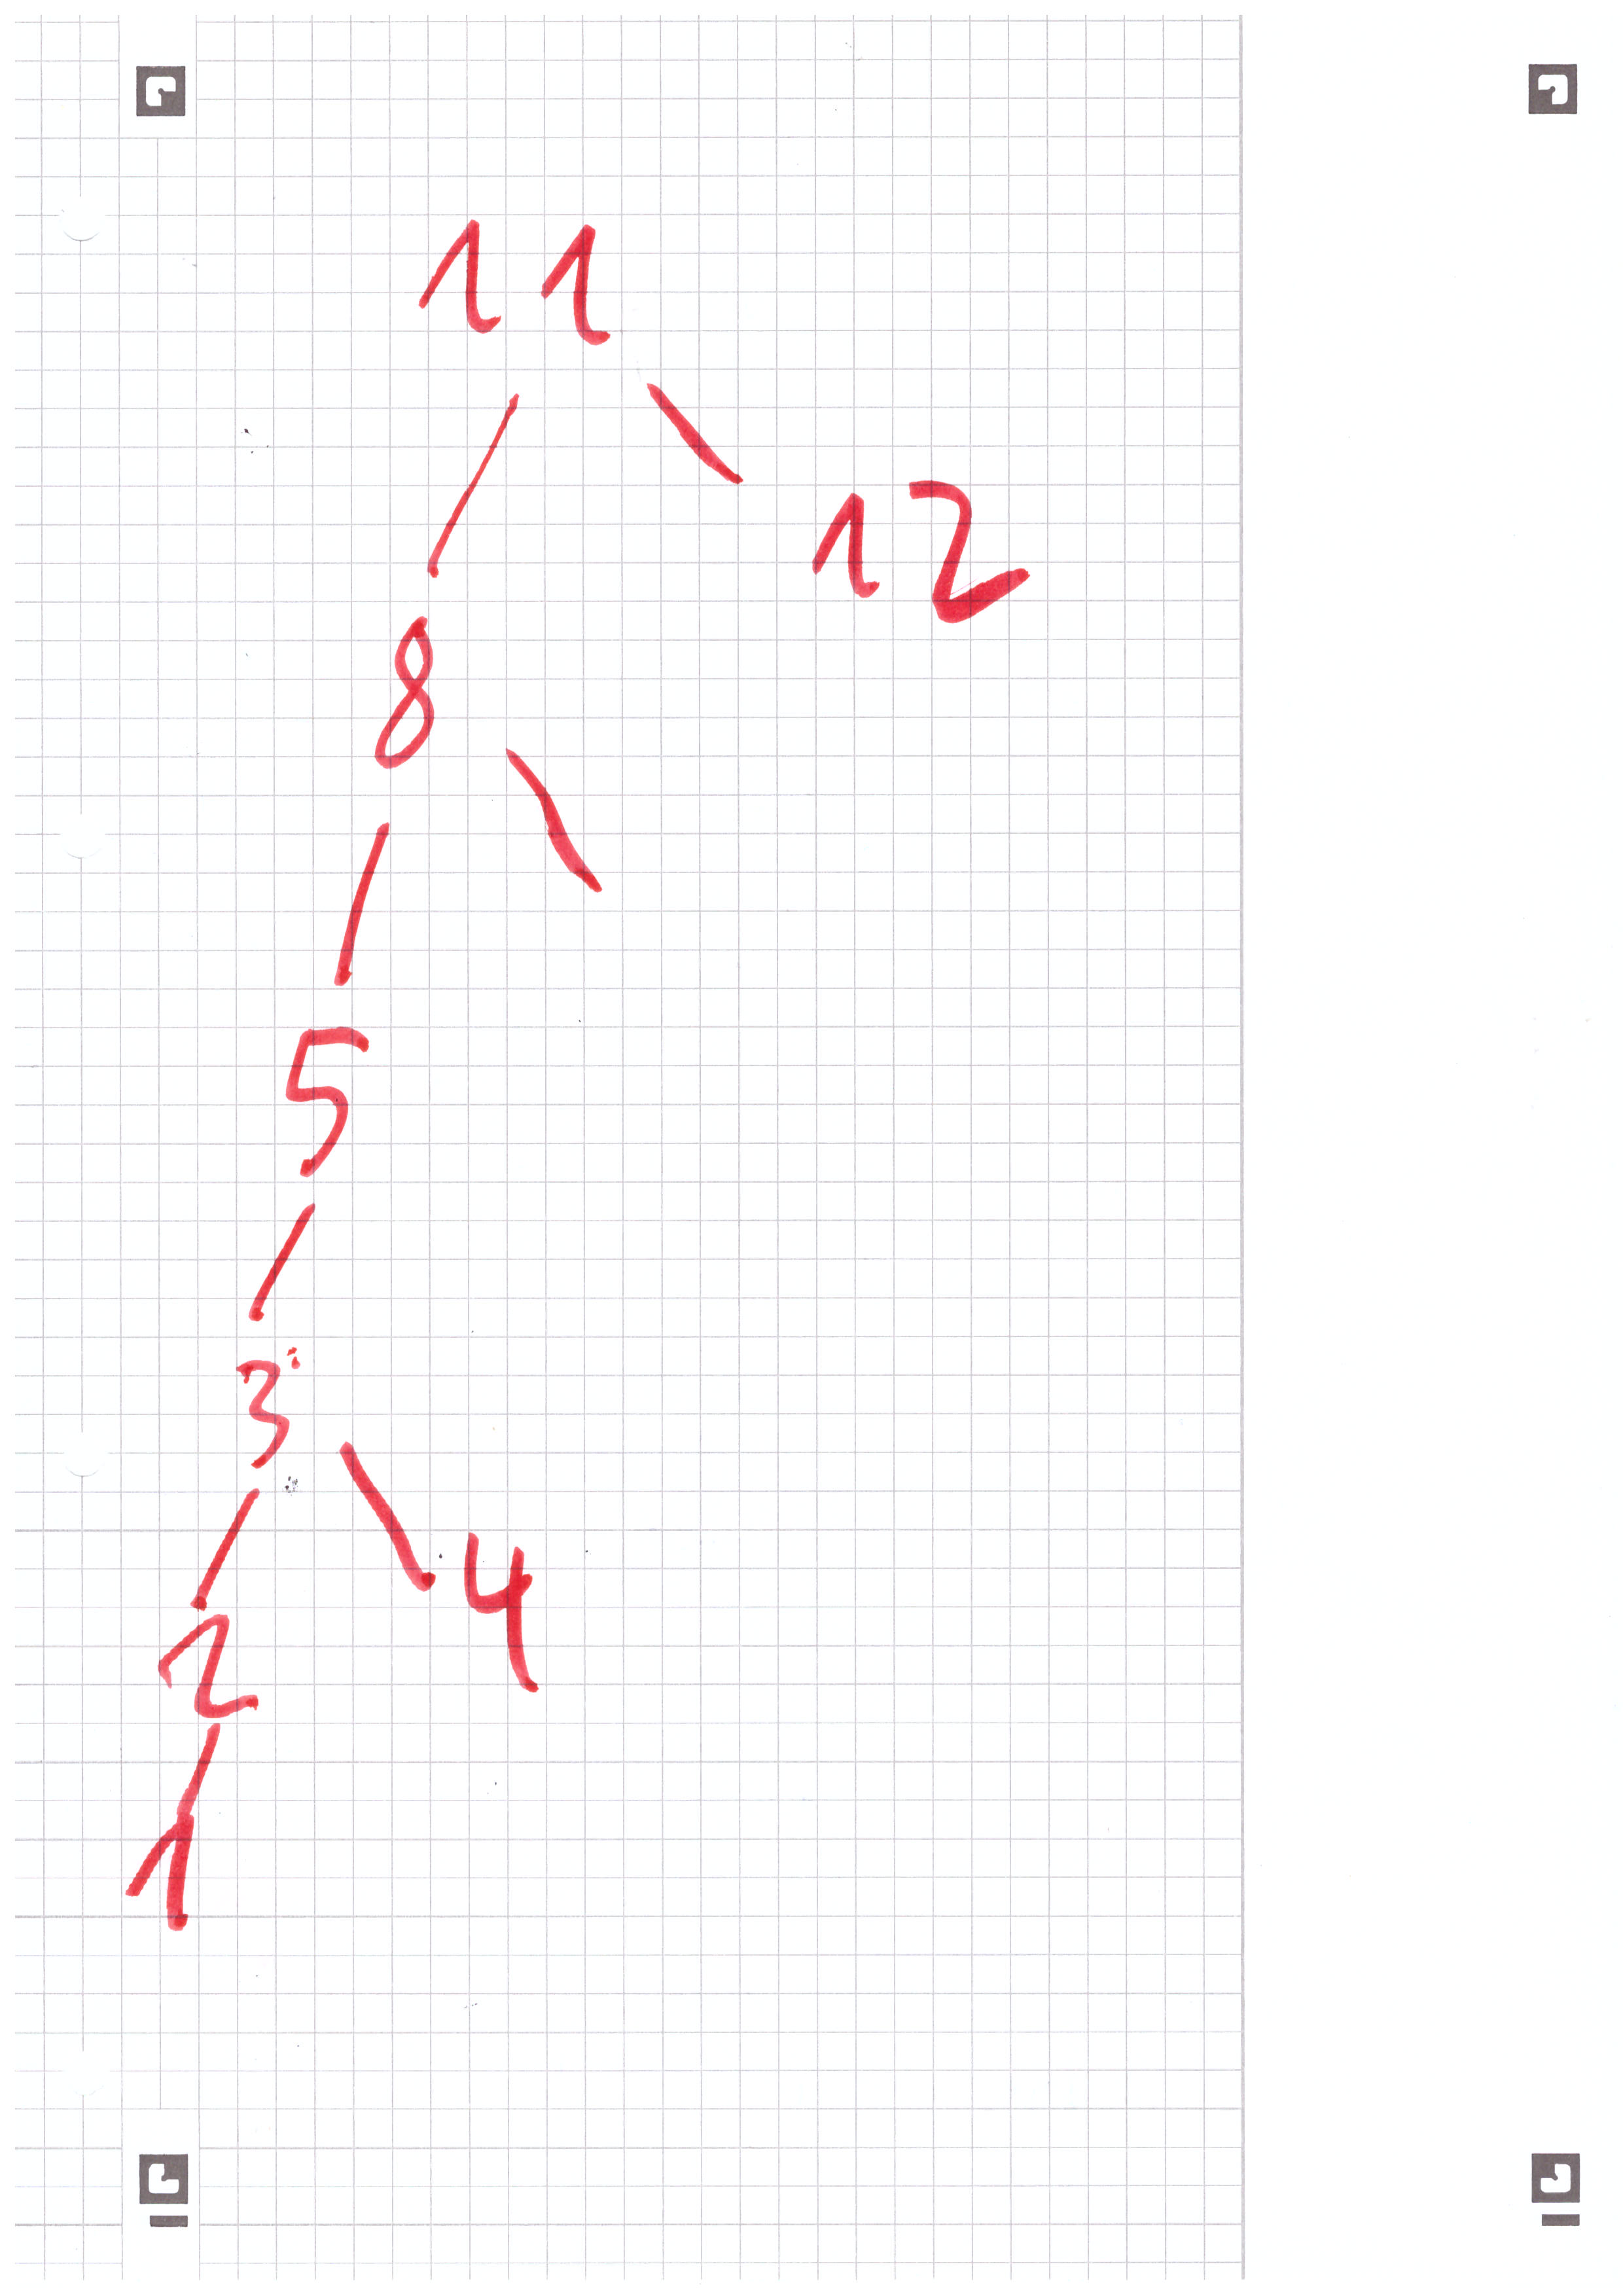
\includegraphics[width=\linewidth]{090102} \\
	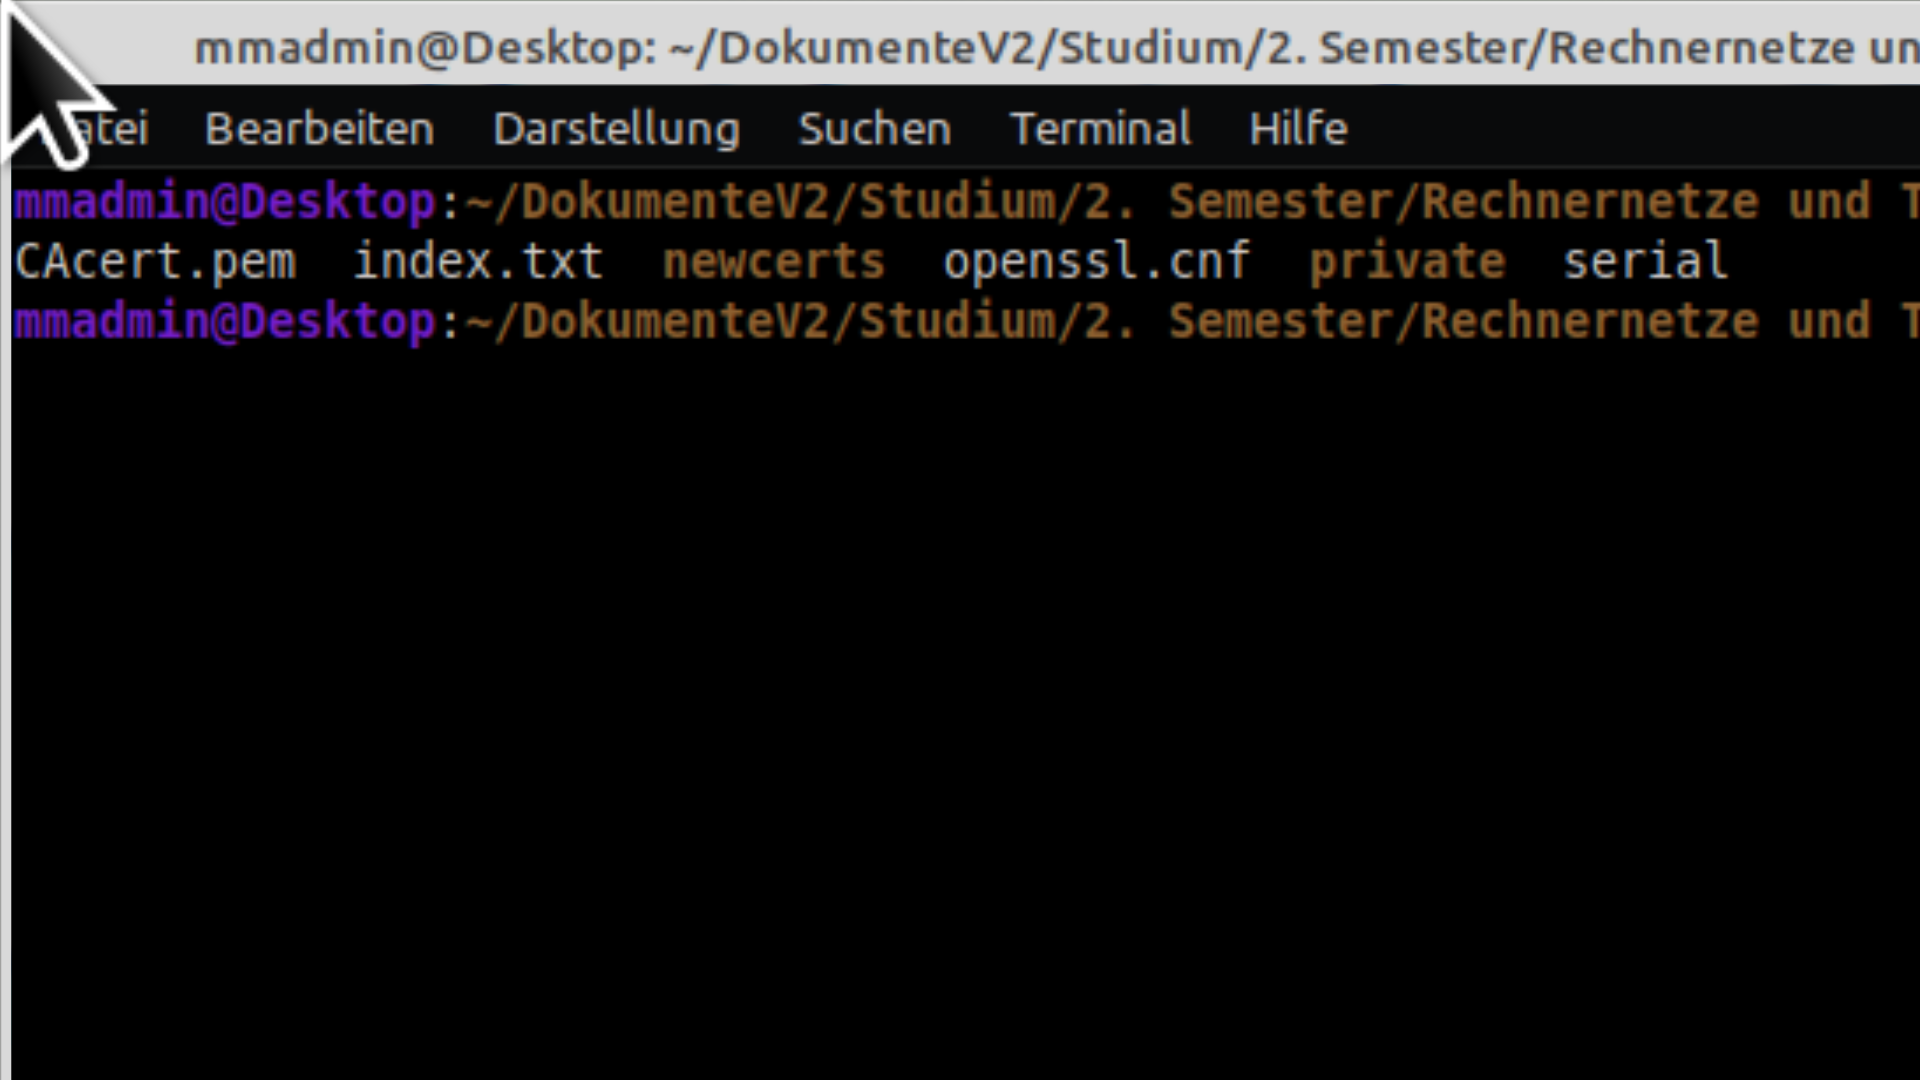
\includegraphics[width=\linewidth]{090103} \\
	RSA Schlüssel erzeugt. \\
	Als Verschlüsselungsalgorithmus dient AES mit einer Schlüssellänge von 128-Bit (AES128). \\
	Das Verfahren gilt als prakmatisch sicher und wird mit höherer Schlüssellänge für das Verschlüsseln geheimer Dokumente verwendet. \\
	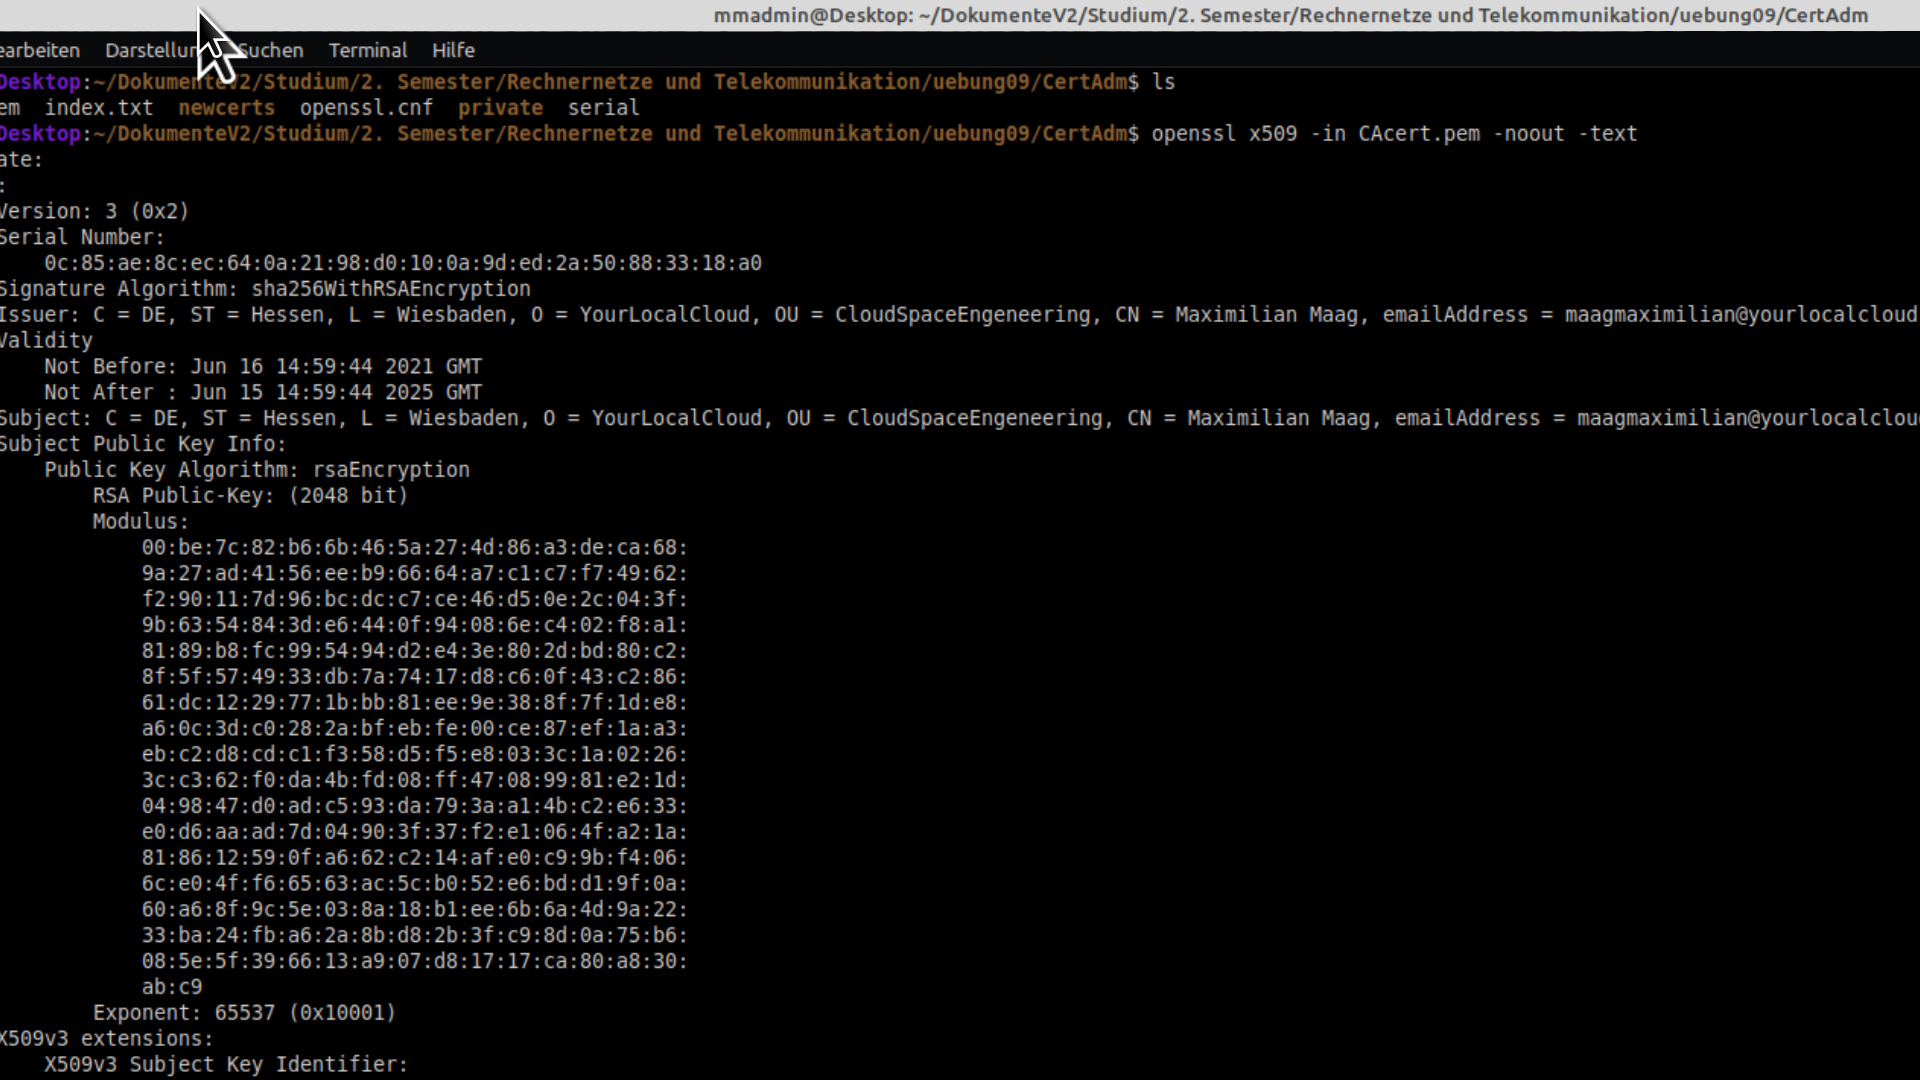
\includegraphics[width=\linewidth]{090104}
	\subsection*{Aufgabe 9.2}
	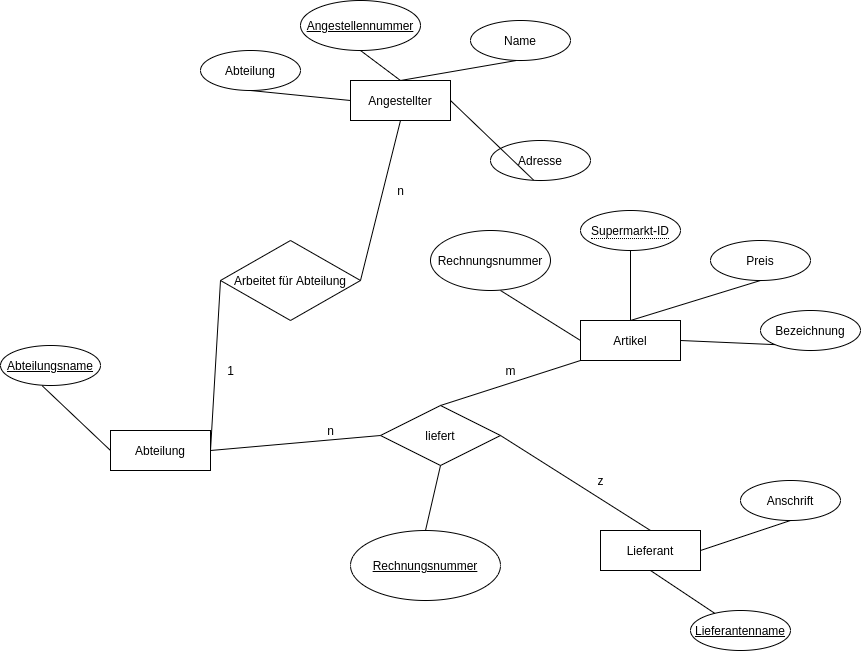
\includegraphics[width=\linewidth]{090201} \\
	Bei der Signierung der Anfrage wird der Private Key des Root-CA verwendet.
	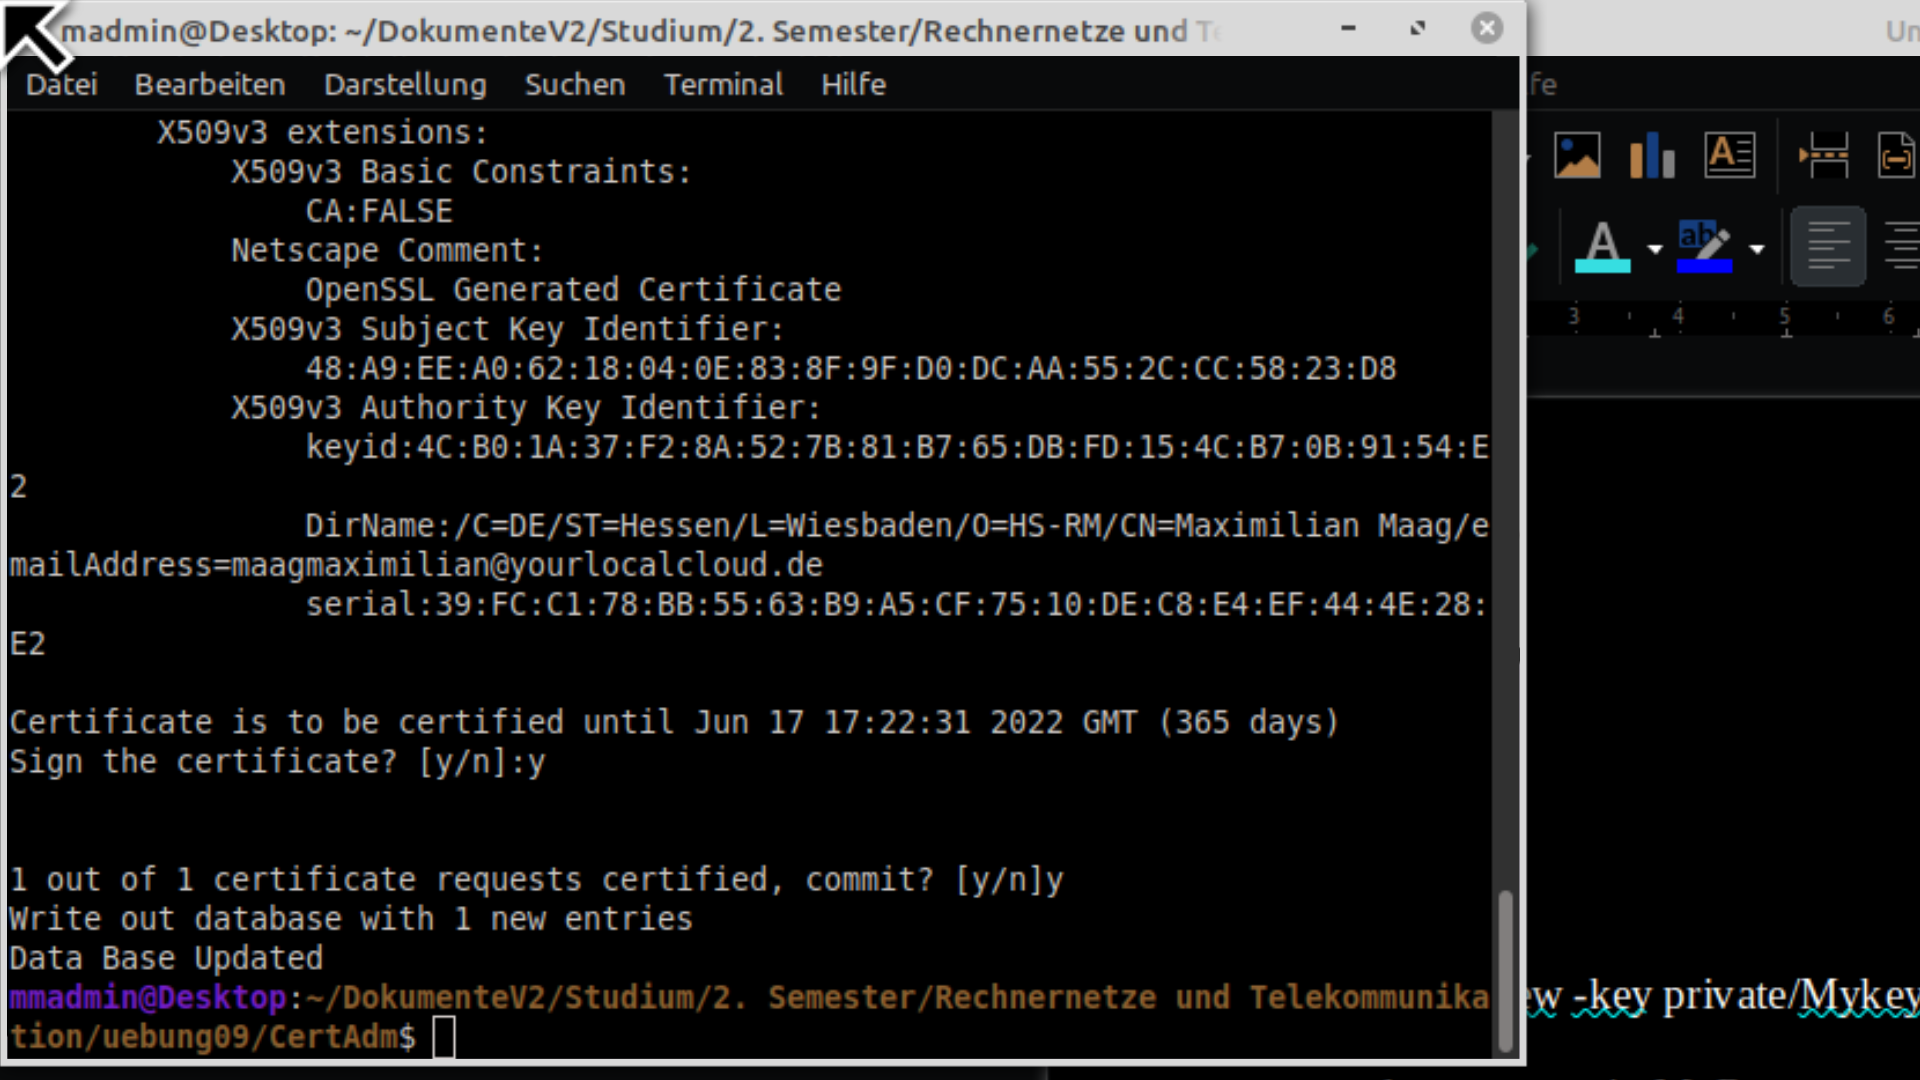
\includegraphics[width=\linewidth]{090202} \\
	Eigenes Zertifikat ausstellen. \\
	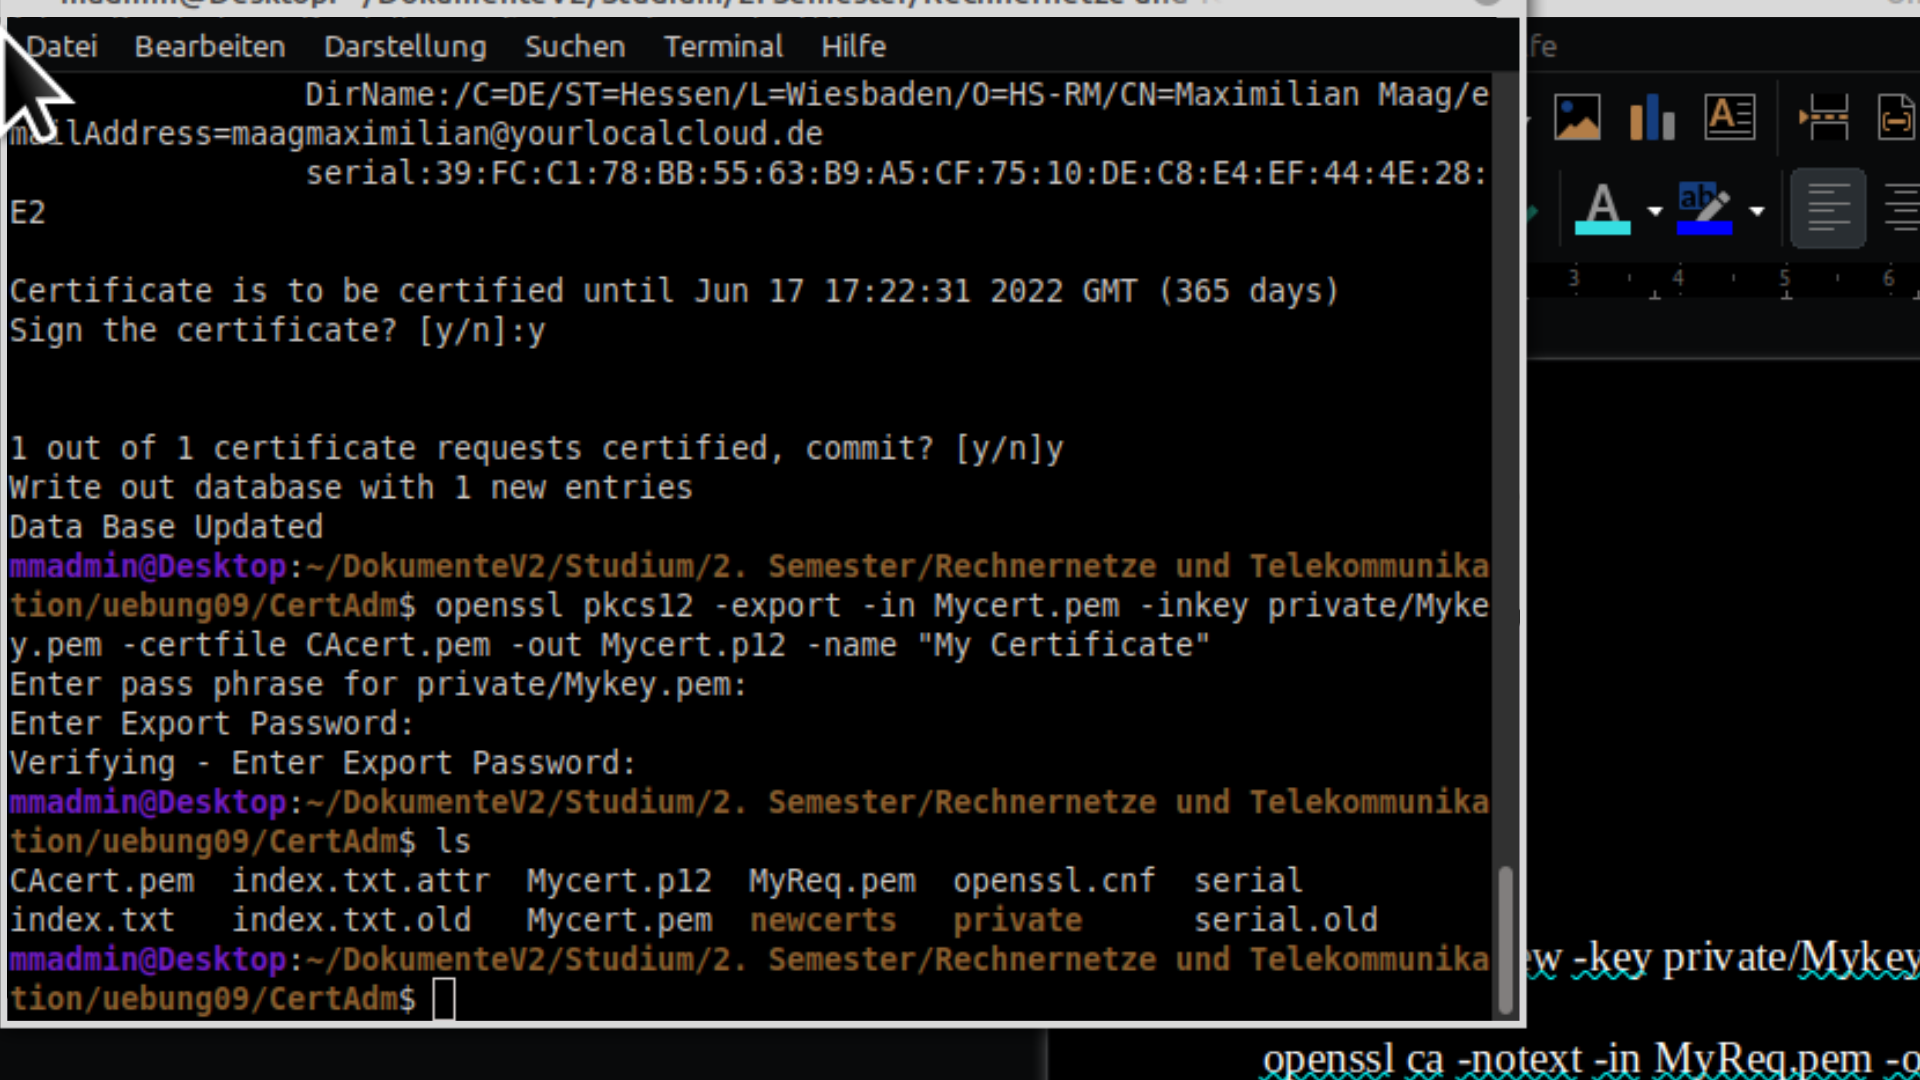
\includegraphics[width=\linewidth]{090203}
	\subsection*{Aufgabe 9.3}
	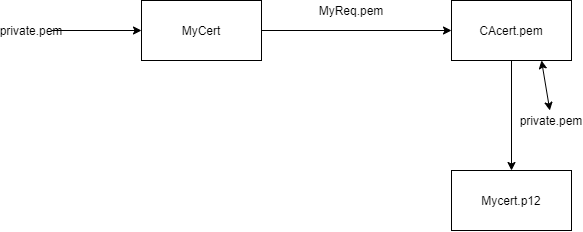
\includegraphics[width=\linewidth]{090301}
	\subsection*{Aufgabe 9.4}
	Der Empfänger der E-Mail muss dem von mir ausgestellten Root-CA trauen. \\
	Für eine besonders sichere E-Mail benötige ich den öffentlichen Schlüssel des Empfängers. 
	Das stellt sicher, dass der Inhalt nur vom Empfänger gelesen werden kann.
\end{document}